% -------------------------------------- PREAMBLE STARTS HERE --------------------------------------------
% This is the preamble. It sets the main options for your document and load the packages used.

% Load packages: making changes here can cause errors.
\documentclass{article}                 % Define document class. Shouldn't change.
\usepackage{booktabs}
\usepackage{tabularx}
\usepackage{import}                     % This package allows us to import files.
\usepackage{multirow}
\usepackage{adjustbox}                  % This package allows you to adapt table and figure sizes to fit the page and is required by iebaltab
\usepackage{geometry}
\usepackage{subcaption}                 % This packages is used to create subfigures
\usepackage{float}

\usepackage{setspace}
\doublespacing                          % Comment out (write % at the beginning of the line) to use single spacing
\usepackage{indentfirst}	            % Indents the fist paragraph of each section
\usepackage{parskip}                    % This packages sets the spacing between two paragraphs
\setlength{\parskip}{.5\baselineskip}   % Define spacing between two paragraphs


% ADD YOUR PROJECT INFO HERE
\title{DIME template for \LaTeX \\ Importing tables} 	% Double backslash starts a new line in \LaTeX
\author{Luiza Andrade \& Mrijan Rimal}
%\date{}                    							% Uncomment this to not print date or insert specific date

% -------------------------------------- PREAMBLE ENDS HERE --------------------------------------------


\begin{document}            % Will not compile without this line

    \maketitle
    \tableofcontents        % Comment out to not print summary
    \listoffigures			% Comment out to not print the list of figures

    \newpage
    \section{Introduction} %The titles are created automatically after using this command. This command is also useful as you can create a table of content just by using this. There is no need to do anything extra.

        This template was created to make your life easier. You should be able to create a PDF file with the figures you generated by just editing the path to the files you exported from Stata.

    \section{Figures}

         % Edit the path after \includegraphics to match the location of your figure. You can also edit the figure size by using [width=\linewidth]. Typing .5 \linewidth before will reduce it to half the size, and typing .8 to 80% and so on.
		\begin{figure}[H]
			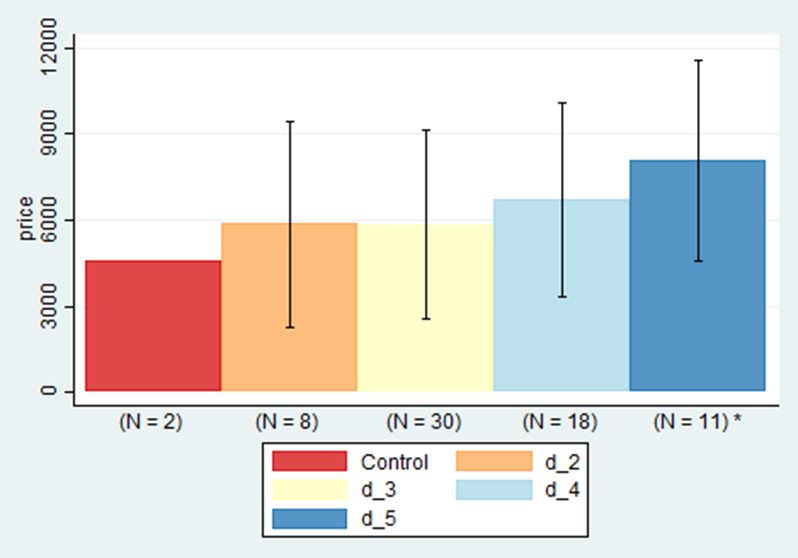
\includegraphics{../Raw/iegraph}
		\end{figure}


\end{document}      % Will not compile without this line
